\chapter{EUDAQ Parameters}\label{ch:EUDAQPar}
List of parameters that are parsed by the EUDAQ run control \gls{gui} to configure the \gls{tlu}.\\
The parameters must be included in the INI or CONF file passed to the main window (see~fig.\ref{fig:EUDAQGui}).
\begin{figure}
  \centering
  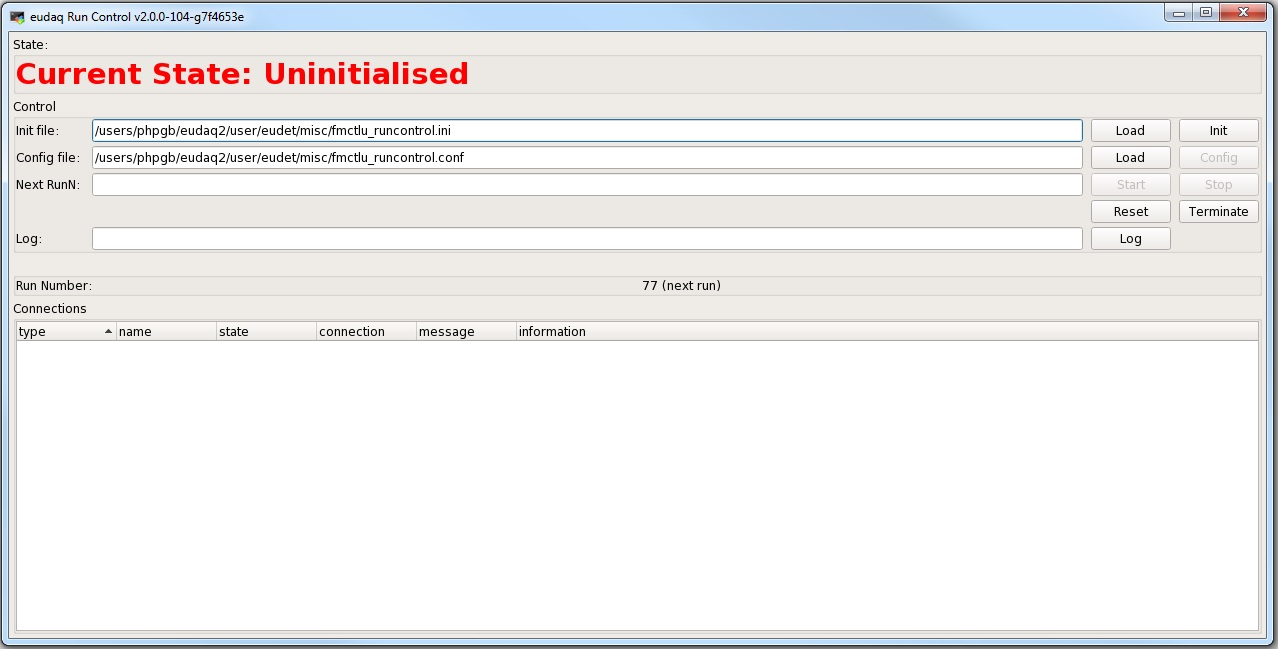
\includegraphics[width=.90\textwidth]{./Images/RunControlGUI.jpg}
  \caption{Main user iterface of the EUDAQ framework.}
  \label{fig:EUDAQGui}
\end{figure}\\
Not all parameters are needed; if one of the parameters is not present in the files, the code will generally assume a default value, indicated in brackets in the following document \verb|[type, default]|.
\section{INI file}
\begin{description}
  \item[initid] \verb|[string, "0"]| Does not serve any purpose in the code but can be useful to identify configuration settings used in a specific run. EUDAQ will store this information in the run data.
  \item[ConnectionFile] \verb|[string, "file://./FMCTLU_connections.xml"]| Name of the xml file used to store the information required to communicate with the hardware, such as its IP address and the location of the address map. The default location indicates a file that must be located in the \texttt{bin} folder.
  \item[DeviceName] \verb|[string, "fmctlu.udp"]| The name of the type of hardware to be contacted by the IPBus.
  \item[TLUmod] \verb|[string, "1e"]| Version of the \gls{tlu} hardware. Reserved for future use.
  \item[nDUTs] \verb|[positive int, 4]| Number of \gls{dut} in the current \gls{tlu}. This is for future upgrades and should not require editing by the user.
  \item[nTrgIn] \verb|[positive int, 6]| Number of trigger inputs in the current \gls{tlu}. This is for future upgrades and should not require editing by the user.
  \item[I2C\_COREEXP\_Addr] \verb|[positive int, 0x21]| \gls{i2c} address of the core expander mounted on the Enclustra board. This is not required if a different \gls{fpga} is used.
  \item[I2C\_CLK\_Addr] \verb|[positive int, 0x68]| \gls{i2c} address of Si5345 clock generator installed on the \gls{tlu}.
  \item[I2C\_DAC1\_Addr] \verb|[positive int, 0x13]| \gls{i2c} address of \gls{dac} installed on the \gls{tlu}. The \gls{dac} is used to configure the threshold of the trigger inputs.
  \item[I2C\_DAC2\_Addr] \verb|[positive int, 0x1F]| \gls{i2c} address of \gls{dac} installed on the \gls{tlu}. The \gls{dac} is used to configure the threshold of the trigger inputs.
  \item[I2C\_ID\_Addr] \verb|[positive int, 0x50]| \gls{i2c} address the unique ID \gls{eeprom} installed on the \gls{tlu}. The chip is used to provide a unique identifier to each kit.
  \item[I2C\_EXP1\_Addr] \verb|[positive int, 0x74]| \gls{i2c} address the bus expander used to select the direction of the \gls{hdmi} pins on the board.
  \item[I2C\_EXP2\_Addr] \verb|[positive int, 0x75]| \gls{i2c} address the bus expander used to select the direction of the \gls{hdmi} pins on the board.
  \item[intRefOn] \verb|[boolean, false]| If true, the \gls{dac}s installed on the \gls{tlu} will use their internal voltage reference rather than the one provide externally.
  \item[VRefInt] \verb|[float, 2.5]| Value in volts for the internal reference voltage of the \gls{dac}s. The voltage is chosen by the chip manufacturer. This is only used if \verb|intRefOn= true|.
  \item[VRefExt] \verb|[float, 1.3]| Value in volts for the external reference voltage of the \gls{dac}s. The voltage is determined by a circuit on the \gls{tlu} and the value of this parameter must reflect such voltage. This is only used if \verb|intRefOn= false|.
  \item[CONFCLOCK] \verb|[boolean, true]| If true, the clock chip Si5345 will be re-configured when the INIT button is pressed (see figure~fig.\ref{fig:EUDAQGui}). The chip is configured via \gls{i2c} interface using a specific text file (see next parameter). After a power cycle, the chip is not configured and must be reconfigured to operate the \gls{tlu} correctly.
  \item[CLOCK\_CFG\_FILE] \verb|[string, "./../user/eudet/misc/fmctlu_clock_config.txt"]| Name of the text file used to store the configuration values of the Si5345. The file can be generate using the Clockbuilder Pro software provided by \href{https://www.silabs.com/products/development-tools/software/clock}{SiLabs}.
\end{description}

\section{CONF file}
\begin{description}
  \item[confid] \verb|[string, "0"]| Does not serve any purpose in the code but can be useful to identify configuration settings used in a specific run. EUDAQ will store this information in the run data.
  \item[verbose] \verb|[int, 0]| Defines the level of output messages from the \gls{tlu}. 0 indicates minimum output.
  \item[HDMI1\_set] \verb|[unsigned int, 0b0001]| Defines the source of the signal on the pins for the \verb|HDMI1| connector. A 1 indicates that each pin pair is an driven by the \gls{tlu}, a 0 that they are left floating (with respect to the \gls{TLU}). This can be used to define the signal direction on each pin pair. The order of the pairs is as follow:\\
  bit 0= CONT, bit 1= SPARE, bit 2= TRIG, trig 3= BUSY. Note that the direction of the DUTClk pair is defined in a separate parameter.\\
  Example to configure the connector to work with an EUDET device:\\
  - in this configuration the BUSY line is driven by the device under test, so it is an input for the \gls{tlu} and should not be driven by it (bit 3= 0)\\
  - TRIGGER line is an output for the \gls{tlu} so is driven by the it (bit 2= 1)\\
  - SPARE line is currently not used and can be configured in either direction. However, future use is likely to have it configured as driven by the \gls{tlu} (bit 1= 1)\\
  - CONT is used by the \gls{tlu} to issue control commands and should be configured as an output (bit 0= 1).\\
  Therefore the value of this parameter would be 0x7 (b1110).
  \item[HDMI2\_set] \verb|[unsigned int, 0b0001]| Defines the direction of the pins for the \verb|HDMI2| connector.
  \item[HDMI3\_set] \verb|[unsigned int, 0b0001]| Defines the direction of the pins for the \verb|HDMI3| connector.
  \item[HDMI4\_set] \verb|[unsigned int, 0b0001]| Defines the direction of the pins for the \verb|HDMI4| connector.
  \item[HDMI1\_clk] \verb|[unsigned int, 1]| Defines if the DUTClk pair on the \gls{hdmi} connector must be driven by the \gls{tlu} and, if so, what clock source to use. A 0 indicates that the pins are not driven by the \gls[tlu}. 1 indicates that pins will by driven with the clock produced from the on-board clock chip Si5345. 2 indicates that the driving clock is obtained from the \gls{fpga}.\\
      Example to configure the connector to work with an EUDET device: in this scenario the clock is driven by the \gls{dut} so the parameter should be set to 0.
      Example to configure the connector to work with an AIDA device: in this scenario the clock is driven by the \gls{tlu} so the parameter should be set to either 1 or 2 (by default 1).
  \item[HDMI2\_clk] \verb|[unsigned int, 1]| Defines the driving signal on the corresponding \gsl{hdmi} connector.
  \item[HDMI3\_clk] \verb|[unsigned int, 1]| Defines the driving signal on the corresponding \gsl{hdmi} connector.
  \item[HDMI4\_clk] \verb|[unsigned int, 1]| Defines the driving signal on the corresponding \gsl{hdmi} connector.
  \item[LEMOclk] \verb|[boolean, true]| Defines whether a driving clock is to be provided on the differential LEMO connector of the \gls{tlu}. By default (value= 1), the clock is driven from the clock chip. If the value is set to 0 no clock will be driven.
  \item[in0_STR] \verb|[unsigned int, 0]| Defines the number of clock cycles used to stretch a pulse once a trigger is detected by the discriminator on input 0. This feature allows the user to modify the pulses that are then fed into the trigger logic within the \gls{tlu}.
      A minimum lenght of 6.25~ns is provided if the value is 0. Any extra clock cycle extend the pulse by 6.25~ns (160~MHz clock).
  \item[in0_DEL] \verb|[unsigned int, 0]| Defines the delay, 160~MHz clock cycles, to be assigned to the discriminated pulse from input 0. This can be used to compensate for differences in cable lengths for the signals used to create a trigger.
  \item[in1_STR] \verb|[unsigned int, 0]| Same as \texttt{in1\_STR} but for input 1.   
  \item[in1_DEL] \verb|[unsigned int, 0]| Same as \texttt{in1\_DEL} but for input 1.
  \item[in2_STR] \verb|[unsigned int, 0]| Same as \texttt{in1\_STR} but for input 2.   
  \item[in2_DEL] \verb|[unsigned int, 0]| Same as \texttt{in1\_DEL} but for input 1.
  \item[in3_STR] \verb|[unsigned int, 0]| Same as \texttt{in1\_STR} but for input 3.   
  \item[in3_DEL] \verb|[unsigned int, 0]| Same as \texttt{in1\_DEL} but for input 1.
\end{description} 